\documentclass[10pt]{jsarticle}
\usepackage[dvipdfmx]{graphicx}
\usepackage{braket}
\usepackage{bm,latexsym,amsmath,amssymb,amsfonts,mathrsfs}
\usepackage{tensor}
\usepackage{comment}
%\usepackage{physics}
\usepackage[dvipdfmx,linktocpage=true]{hyperref}
\usepackage{pxjahyper}
\usepackage{color}
\usepackage{here}
\usepackage{tikz}
\usetikzlibrary {arrows.meta}
\usetikzlibrary {bending}
\input{colordvi.tex}

\setcounter{tocdepth}{3}%目次にsubsubsectionまで入れる


\newcommand{\kakko}[1]{\left(#1 \right)} %丸括弧()
\newcommand{\kkakko}[1]{\left[ #1 \right]} %角括弧[]
\newcommand{\nkakko}[1]{\left\{ #1 \right\}} %波括弧{}
\newcommand{\p}[1]{\left| #1 \right|} %縦棒||
\newcommand{\henbi}[2]{{\frac{\partial#1}{\partial#2}}} %偏微分
\newcommand{\bi}[2]{{\frac{d #1}{d #2}}} %微分

\newcommand{\del}{{\partial}} %偏微分の∂
\newcommand{\skakko}[1]{$\ll$#1$\gg$}
\newcommand{\vc}[1]{\overrightarrow{#1}}% 矢印ベクトル
\newcommand{\vct}[1]{\bm{#1}}%太字ベクトル
\newcommand{\sint}[1]{\int\mathcal{D}#1\,}%経路積分
\newcommand{\pms}[1]{\mathcal{D}#1\,}%経路積分の測度

%\newcommand{\Res}{\mathrm{Res}}
\renewcommand{\Im}{\mathrm{Im\,}}
\renewcommand{\Re}{\mathrm{Re\,}}
\DeclareMathOperator*{\Res}{Res}

\renewcommand{\theenumi}{\Alph{enumi}}
\renewcommand{\labelenumi}{(\theenumi)}

\numberwithin{equation}{section}%数式番号を(n.m)の形で書く。

\topmargin=0.0in
\headsep=0.0in
\headheight=0.0in
\oddsidemargin=-0.22in
\evensidemargin=-0.22in
\textwidth=6.5in
\textheight=9.0in
\title{AI入門としての線形代数}
\author{TiroDuetto}
\date{\today}
\pagestyle{empty}
\begin{document}
\maketitle

\begin{abstract}
表題にはAI入門と銘打ってあるが私がAIについて詳しくないので、ほとんど線形代数の基本的な部分を記す。
一応計算機による解析も勉強していくつもりであり、このノート内でもできる限り具体例を提示していきたい。
内容はまだ書きかけなので随時更新していく。
もし重大な誤植や論理の間違いがあれば指摘してほしい。
なお、コンピュータとを計算機と呼んでいるのはそういう文化の人間が作った資料であるためであって深い意味はない。ゆえに表現が統一されていないところもあると思う。
このノートでは「我々が扱う空間は3次元Euclid空間であり、これは内積の定義された計量ベクトル空間である」という文章が理解できるところまで進めたら幸いと思う。
また、目次の5章と6章あたりの内容まで理解できれば計算機を用いた機械学習などにも応用できるだろうと期待している。
\end{abstract}
\tableofcontents
\setcounter{section}{-1}
\section{数学的記法における注意}
\subsection{集合}
対象物の集まりを{\bf 集合}という。その集合を構成する対象物のことを{\bf 元}や{\bf 要素}という。集合$A$に元$a$が属することを
\begin{equation}
  a \in A 
\end{equation}
と書く。またすべてが$A$の元からなる集合$B$のことを、$A$の部分集合といい、
\begin{equation}
  B \subset A
\end{equation}
と書く。
\subsubsection{数の集合}
ある数全体の集合には特別な記号が用意されている。複素数$\mathbb{C}$, 実数$\mathbb{R}$, 有理数$\mathbb{Q}$, 整数$\mathbb{Z}$, 自然数$\mathbb{N}$など。
なお、この書体は黒板太字と呼ばれ、通常出版物において単なる太字である字を黒板で書くときに使われるが、以上の例のように特別な意味を持たせることもある。
もちろん出版物においては通常の太字で書いても問題はない。
例えば実数全体の集合を{\bf R}のように表している書籍もある。
\subsubsection{直積}
$c \in C, \, d\in D$を用いた$(c,d)$全体の集合のことを$C$と$D$の{\bf 直積}といい、$C\times D$と表す。例えば、座標平面上の点$(x,y)$は$\mathbb{R}\times \mathbb{R}$の元であると言える。なお、$\mathbb{R}\times \mathbb{R}=\mathbb{R}^{2}$とも書く。
\subsection{写像}
2つの集合があるとき、一方の集合の元に対して、もう一方の集合の元がただひとつに定まるような関係付けの規則を{\bf 写像}という。 
集合$V$から集合$W$への写像$f$を
\begin{equation}
  f:V \to W
\end{equation}
のように書く。あるいは元どうしの関係で$v\in V, \, w\in W$として
\begin{equation}
  v \mapsto w= f(v)
\end{equation}
と書く。$v \mapsto f(v)$と書いてもよい。大雑把に言えば$v$を入力したら$f$という規則によって$w$が出力されるということである。特に$V$や$W$が数の集合であれば、{\bf 関数}と呼ばれる。
\paragraph{例}
\begin{description}
  \item[実数から実数] 関数$y=f(x)$を以上の記法で表すと
  \begin{equation}
   f:\mathbb{R}\to\mathbb{R}, \quad x\mapsto y=f(x)
  \end{equation}
 \item[実数から複素数] 虚数単位$i=\sqrt{-1}$を用いて、$(x,y)\in \mathrm{R}^{2}$から複素数$z\in \mathbb{C}$を$z=g(x,y)=x+iy$のように定める。
 \begin{equation}
  g:\mathbb{R}^{2}\to \mathbb{C},\quad (x,y)\mapsto z=x+iy
 \end{equation}
 
\end{description}
\section{線形代数とは何か?}
世の中を大まかに把握したいとき、その現象を''真っ直ぐなもの''や''平らなもの''とみなしたり、単なる比例関係として扱うと便利だ。
例えば球体である地上に暮らしていても自分の近傍を平面とみなしたり、アルバイトによる収入も「毎月この程度」と簡単に近似して計算するだろう。
こういった考え方を「線形的に近似する」などと表現する。記憶にありそうな例で言えば、比例やその発展である1次関数である。
つまり、名前の通り「線形的な」対称を研究するのが線形代数というわけである。
また、代数という言葉は、簡単に言えば文字式による計算や方程式の研究する分野に用いられる。
合わせて「1次関数を研究する」学問と思っていて貰えばよい。
物理学においては本質的に非線形な現象であったとしても、そのうちの線形な部分を切り出して現象を理解したり、あるいは理論を構築していく。
\subsection{計算機において}
もともとはそういった動機から活かされていたのであるが、線形代数は奥が深く、応用範囲の広い分野である。
その重要な対称が{\bf ベクトル}や{\bf 行列}である。
今回の本題である計算機による解析では、いくつものデータをベクトルとして扱い、また新たなデータへの変換やその関係を行列で表す。$n$個のデータを$n$成分ベクトルで次のように表すとしよう
。\footnote{わかりやすさのために矢印でベクトルを表しているが、$\vc{v}$以外にも太字の$\vct{v}$やあるいは先にベクトルであると宣言した上で通常の$v$のまま表すこともある。物理をやっている人はこのあたりにこだわりがあるらしく、3次元は太字や矢印、4次元以上は特に明示せず、量子力学の文脈では$\ket{v}$などと書く。}
\begin{equation}
  \vc{v}=\left( \begin{matrix}
    v_{1}\\
    \vdots \\
    v_{n}
  \end{matrix} \right)
\end{equation}
このベクトルを$m$個のデータを表すベクトル$\vc{u}$に変換すると考える。
\begin{equation}
  \vc{v}=\left( \begin{matrix}
    u_{1}\\
    \vdots \\
    u_{m}
  \end{matrix} \right)
\end{equation}
単純計算でこの2つをつなげるためには$nm$個の成分を持つ変換が必要であるとわかるだろう。この変換を$A$と書けば
\begin{equation}
  A=\left( \begin{matrix}
    a_{11} & \cdots & a_{1n} \\
    \vdots & \ddots & \vdots \\
    a_{m1} & \cdots & a_{mn}
  \end{matrix} \right)
\end{equation}
これを用いて
\begin{align}
  \vc{u} &= A \vc{v}\\
 \Leftrightarrow  \left( \begin{matrix}
    u_{1}\\
    \vdots \\
    u_{m}
  \end{matrix} \right)&=\left( \begin{matrix}
    a_{11} & \cdots & a_{1n} \\
    \vdots & \ddots & \vdots \\
    a_{m1} & \cdots & a_{mn}
  \end{matrix} \right)\left( \begin{matrix}
    v_{1}\\
    \vdots \\
    v_{n}
  \end{matrix} \right)
\end{align}
このようにベクトル同士規則の変換を表すのが行列である。
そのまま$m\times n$行列と呼ばれる。この$m$や$n$の順序については後ほど説明する。
多数のデータを一度に扱いたい……それをきちんと定式化できたら……という願望を叶えてくれるのがこの計算である。
すでに線形代数で研究されつくされているのだ。
\subsubsection{例}
さて、以上の話は一般論に寄りすぎているし、まだベクトルも行列の話もしていない中では何をしているのか?という疑問のほうが大きいと思われるので簡単な例示をしていく。なお\cite{L-nakanishi}の例を少し改造しただけのものである。
いま、スーパーマーケットにいる。
桃、みかん、りんごの1個あたりの値段・重さの表\ref{momomikan}を知ったとき、果物を買った個数と合計の値段・重さの関係はどのように計算するのだろうか。
\begin{table}[H]
  \centering
  \caption{重さについては平均的な重さと思っておく。(例なのでそこまで重要でもないが)}
  \label{momomikan}
  \begin{tabular}{|c|c|c|c|} \hline
         & 桃 & みかん & りんご  \\ \hline
    値段(円)  & 300 & 100 & 200   \\ \hline
    重さ(g)  & 200 & 30 & 300  \\ \hline
  \end{tabular}
\end{table}


それぞれの果物を1個、2個、5個買ったとする。
もちろんこのときの計算は簡単で
\begin{align}
  (\text{値段})&=300\times 1 + 100\times 2+200\times 5 = 1500\\
  (\text{重さ})&= 200\times 1 + 30\times 2+300 \times 5 = 1760
\end{align}
とできる。これがベクトルと行列を用いれば一つの形式によって表せて便利だという話である。
つまり、
\begin{equation}
  \left( \begin{matrix}
    1500 \\
    1760
  \end{matrix} \right)=\left( \begin{matrix}
    300 & 100 & 200 \\
    200 & 30 & 300
  \end{matrix} \right)\left( \begin{matrix}
   1\\
   2\\
   5
  \end{matrix} \right)
\end{equation}
と表記すればよい。
これも
\begin{equation}
  \vec{x}=\left( \begin{matrix}
    1\\
    2\\
    5
   \end{matrix} \right),\quad A =\left( \begin{matrix}
    300 & 100 & 200 \\
    200 & 30 & 300
  \end{matrix} \right), \quad \vec{y} =\left( \begin{matrix}
    1500 \\
    1760
  \end{matrix} \right)
\end{equation}
と書けば
\begin{equation}
  \vec{y}=A \vec{x}
\end{equation}
の形で書ける。どう見ても1次関数そっくりである。もちろん、この話はやみくもに数字を並べただけでなく、きちんと線形代数の知識に則っている。
勘のいい人は気づいたかもしれないが、結局のところ計算機はこのような計算を繰り返しているということである。

\section{ベクトル}
まず基本的な注意としてベクトルには列ベクトル・行ベクトルがある。同じ$v_{1},\cdots ,v_{n}$を持つベクトルであったとしても
\begin{equation}
  \text{列ベクトル } \vec{a}=\left( \begin{matrix}
    v_{1}\\
    \vdots\\
    v_{n}
  \end{matrix} \right)  \quad , \quad  \text{行ベクトル } \vec{b} = ( v_{1} \quad  \cdots \quad v_{n})\quad 
\end{equation}
の2つは区別される。この関係は$\vec{a}={}^{t}\!\vec{b}$と書ける。以下では全て列ベクトルで記すことにする。
なお、高校数学ではベクトルを$(v_{1},v_{2},\cdots)$のように書いていたがここでの行ベクトルにはカンマ,を入れないことにする。\footnote{ただし、「カンマは書いてはいけない」などと特に決まっているわけではない。人によっては普通に使っていたりする。}

列ベクトルと行ベクトル違いについて、詳しくは行列を学ぶとわかる。
\subsection{基本事項}
{\bf ベクトル}とは大きさと向きを持った量である。例えば、点$O$から点$A$へ向かうベクトルは
\begin{equation}
  \vc{OA}
\end{equation}
とでも書けばよい。決まった表し方があるわけではないのでわかりやすいように書くことをおすすめする。
ではさらに点$A$から点$B$に向かうベクトル$\vc{AB}$を''加える''ことを考えてみよう。
最終的には点$O$を出発して点$B$に向かうベクトルとなることがわかるだろう。これがベクトルの和である。
\begin{equation}
  \vc{OB}=\vc{OA}+\vc{AB}
\end{equation}
 のように表せる。詳しくは後に述べる。
% \begin{figure}[tbh]
%   \begin{minipage}[b]{0.45\linewidth}
%     \centering
%     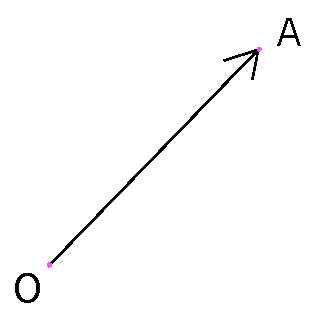
\includegraphics[width=0.8\linewidth]{img/vc-oa.pdf}
%    \caption{ベクトル$\protect \vc{OA} $}%\protectを入れないとなぜかコンパイルが通らない
%     \label{vcoa}
%   \end{minipage}
%   \begin{minipage}[b]{0.45\linewidth}
%     \centering
%     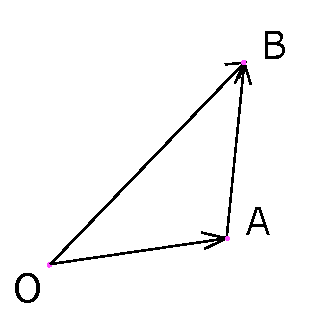
\includegraphics[width=0.8\linewidth]{img/vc-ob.pdf}
%     \caption{ベクトル$\protect \vc{OB}=\protect \vc{OA}+\protect  \vc{AB}$}
%     \label{vcob}
%   \end{minipage}
% \end{figure}


% \begin{figure}[H]
%   \begin{tikzpicture}
%   \draw[->](0,0)--(4,2);
%   \draw(0,0)node[left]{O};
%   \draw(4,2)node[above]{A};
%   \end{tikzpicture}
%   \caption{ベクトル$\protect \vc{OA} $}
% \end{figure}
% \begin{figure}[H]
%   \begin{tikzpicture}
%   \draw[->](0,0)--(2,1);
%   \draw[->](2,1)--(4,3);
%   \draw(0,0)node[left]{O};
%   \draw(2,1)node[above]{A};
%   \draw(4,3)node[above]{B}
%   \end{tikzpicture}
%   \caption{ベクトル$\protect \vc{OB}=\protect \vc{OA}+\protect  \vc{AB}$}
% \end{figure}

\begin{figure}[H]
  \centering
      \begin{tabular}{cc}  
        \begin{minipage}[t]{0.3\linewidth}
          \centering
        \begin{tikzpicture}
          \coordinate (O) at (0,0) node [left] at (O) {O};
          \coordinate (A) at (3,3) node [above] at (A) {A};
      \draw[->](O)--(A);
        \end{tikzpicture}
  \caption{ベクトル$\protect \vc{OA} $}
        \end{minipage} &
        \begin{minipage}[t]{0.3\linewidth}
          \centering
  \begin{tikzpicture}
    \coordinate (O) at (0,0) node [left] at (O) {O};
    \coordinate (A) at (3,1) node [right] at (A) {A};
    \coordinate (B) at (4,3) node [above] at (B) {B};
     \draw[->](O)--(A);
     \draw[->](A)--(B);
     \draw[->](O)--(B);
   \end{tikzpicture}
   \caption{ベクトル$\protect \vc{OB}=\protect \vc{OA}+\protect  \vc{AB}$}
        \end{minipage}
      \end{tabular}
  \end{figure}


また、ここでは特に{\bf 数を並べたもの}と考えることも多い。この2つの表現は当然同じである。
$n$成分をもつベクトル$\vec{v}$は
\begin{equation}
  \vec{v}=\left( \begin{matrix}
    v_{1}\\
    \vdots\\
    v_{n}
  \end{matrix} \right) 
\end{equation}
のように表される。前者の表現のほうが以下に用意する言葉のイメージは付きやすいかもしれない。
向きを持たない量は{\bf スカラー}という。ベクトル$\vec{v}$の大きさを{\bf 絶対値}あるいは{\bf ノルム}と呼び
\begin{equation}
  |\vec{v}| ,\quad \text{あるいは単に細字で}\quad v 
\end{equation}
と書く。$||v||$と2本線で囲むことも多い。数学書ではだいたいこう書かれる。大きさは向きを持たないのでスカラーである。大きさが同じで、向きが全く逆方向のベクトルを逆ベクトルと呼び
\begin{equation}
  -\vec{v}
\end{equation}
と負号を添えて書く。2つのベクトル$\vec{v},\, \vec{w}$の大きさと向きがどちらも同じとき、これらのベクトルは{\bf 等しい}といって
\begin{equation}
  \vec{v} = \vec{w}
\end{equation}
と表す。これは両方のベクトルの各成分が等しいことを意味する。
構成する数が同じであったとしても順番が違えば違うベクトルである。
\begin{equation}
  \left( \begin{matrix}
    1\\
    2\\
    3
  \end{matrix} \right) \neq\left( \begin{matrix}
    1\\
    3\\
    2
  \end{matrix} \right)
\end{equation}
大きさが1のベクトルを{\bf 単位ベクトル}と呼ぶ。例えば$\vec{v}$の方向の単位ベクトルは
\begin{equation}
  e_{\vec{v}}=\frac{\vec{v}}{|v|}
\end{equation}
と表せる。これのことは方向ベクトルとも呼ぶ。なお、方向を指定しないで単位ベクトルと言っても意味がないので注意。
大きさが0のベクトル、すなわち全ての成分が0であるベクトルは{\bf ゼロベクトル}と呼ばれ、$\vec{0}$で表される。単に$0$と表すこともある。
\begin{equation}
  \vec{0}=\left( \begin{matrix}
    0\\
    0\\
    \vdots \\
    0
  \end{matrix} \right)
\end{equation}
また、空間中の点も数を並べて表現されていたので、この点を{\bf 位置ベクトル}という言葉で表せる。例えば3次元空間上の点について
\begin{equation}
    (x,y,z) \quad \leftrightarrow \quad \left( \begin{matrix}
      x\\
      y\\
      z
    \end{matrix} \right)
\end{equation}
で表すことができる。
\subsubsection{演算}
スカラー倍と2つのベクトルの和、内積を定義する。商は定義されない。
成分の数が違うときは和や積を定義できないことに注意。
なお、単に積ではなく内積という言葉を用いたのは外積と呼ばれる積もあるためである。
外積はあとでやるかも。
\begin{description}
  \item[スカラー倍] あるベクトル$\vec{v}$をスカラー$a$倍したとき、各成分が$a$倍される。
  \begin{equation}
    a\vec{v}=\left( \begin{matrix}
      av_{1}\\
      \vdots \\
      av_{n}
    \end{matrix} \right)
  \end{equation}
  図的な表現をすれば$a>0$ならば向きは同じで大きさが$|a|$倍され、$a<0$ならば向きは反対で大きさが$|a|$倍されたベクトルとなる。
  \item[和] 2つのベクトルの和は各成分ごとに和を取るものとする。例えば
  \begin{equation}
    \left( \begin{matrix}
      a\\
      b\\
      c
    \end{matrix} \right)+\left( \begin{matrix}
      d\\
      e\\
      f
    \end{matrix} \right)=\left( \begin{matrix}
      a+d\\
      b+e\\
      c+f
    \end{matrix} \right)
  \end{equation}
  である。先に少し述べたような図の描像では、始点から途中の点を介して終点まで向かうように描かれ、最終的には単に始点から終点へ向かうベクトルとなる。
  なお、差については$(-1)$倍して足したと考えるとよい。
  \begin{equation}
    -\vec{v}=(-1)\vec{v}
  \end{equation}
  先に紹介した逆ベクトルとは足したらゼロベクトルになるベクトルとして定義される。
  ゼロベクトルは足しても引いてももとのベクトルは変わらない
  。\footnote{群論の言葉では演算してももとの形のままとなる元を単位元、足して単位元となる元を逆元と呼ぶ。ここでは単位ベクトルとの言葉遣いが紛らわしいのであまり使わないようにする。}
  \item[内積] ベクトル特有の演算である。これは2つのベクトルからスカラーを作り出すものである。$\vec{v},\vec{w}$を$n$成分のベクトルとすると
  \begin{equation}
    \vec{v}\cdot \vec{w} = v_{1}w_{1}+\cdots + v_{n}w_{n}=\sum_{i=1}^{n}v_{i}w_{i}
  \end{equation}
と定義される。内積を$(\vec{v},\vec{w})$や$\braket{\vec{v},\vec{w}}$で表すこともある。ベクトルのノルムはこの内積を用いて定義され、
\begin{equation}
  |\vec{v}|=\sqrt{\vec{v}\cdot \vec{v}}
\end{equation}
である。また、2つのベクトルのなす角$\theta$とすると
\begin{equation}
  \vec{v}\cdot \vec{w}=|\vec{v}||\vec{w}|\cos{\theta}
\end{equation}
と書ける。この書き方についてはきちんと図的な表し方から納得できることを確認してほしい。
\end{description}
また、以上に関係する諸概念についても紹介する。
\paragraph{距離}ベクトルどうしの距離を定義したい。


まず{\bf 距離}というものを少し堅苦しい書き方ではあるが定義しておく。読み飛ばしても差し支えはない。集合$X$について距離関数
\begin{equation}
  d:X\times X \to \mathbb{R}
\end{equation}
は任意の$X$の元$x,y,z$について以下の条件を満たす。
\begin{enumerate}
  \item $d(x,y)\geq 0$(非負性)
  \item $d(x,y)=d(y,x)$(対称律)
  \item $x=y$のときのみ$d(x,y)=0$
  \item $d(x,y)\leq d(x,z)+d(z,y)$(三角不等式\footnote{劣加法性とも言う。})
\end{enumerate}
ここでは、ベクトルどうしの距離の定義として{\bf Euclid距離}を用いる。すなわち、$\vc{v},\vc{w}$に対して
\begin{equation}
  \label{kyori}d(\vc{v},\vc{w})=\sqrt{|v_{1}-w_{1}|^{2}+\cdots +|v_{n}-w_{n}|^{2}}
\end{equation}
位置ベクトルの考え方を思い出せば、これは単に2点間の距離を表しているにすぎないことがわかる。
三平方の定理の$n$次元への一般化である。
このように定義した距離が上の条件$1.\sim 4.$を満たすことを確認しておこう。
\paragraph{コサイン類似度}
2つのベクトルがどれだけ''近いか''を図る尺度として{\bf コサイン類似度}を定義できる。ベクトル$\vc{v},\vc{w}$に対してコサイン類似度$\mathrm{sim}(\vc{v},\vc{w})$を
\begin{equation}
\label{cossim} \mathrm{sim}(\vc{v},\vc{w})=\frac{\vc{v}\cdot \vc{w}}{|\vc{v}||\vc{w}|}=\cos{\theta}
\end{equation}
によって定める。これは$-1\leq \mathrm{sim}(\vc{v},\vc{w})\leq 1$で''近さ''を判定するものである。例えば$\mathrm{sim}(\vc{v},\vc{w})=1$であれば$\cos{\theta}=1$、すなわち$\theta=0$なので全く同じ方向を向いていて、コサイン類似度の観点からは最も''近い''といえる。
反対に、$\mathrm{sim}(\vc{v},\vc{w})=-1$であれば$\cos{\theta}=-1$、すなわち$\theta=\pi$であるから、全く逆方向に向いているベクトルである。
このとき最も''遠い''と思えるだろう。
なお、定義から分かる通り、コサイン類似度はベクトルの大きさは関係なく、角度で近さを測っている。
\subsubsection{位置ベクトル}
ベクトルと座標の関係をもう少し詳しく説明する。
もともとベクトル自体は座標系によらない量\footnote{直交座標を使おうが極座標を使おうがその矢印そのものは全く変わらずそこに''在る''ため。}であるが、座標を指定すると計算において便利である。


$xy$平面上で図\ref{Aab}のようにA$(a,b)$という点があったとする。
この数字の意味するところはもちろん、「$x$軸方向に$a$だけ進み、$y$軸方向に$b$だけ進んだところ」と解釈する。そして、ベクトル$\vc{OA}$を位置ベクトルとして、点Aを表すものと考える。
\begin{equation}
  A(a,b)\quad\leftrightarrow\quad \vc{OA}=\left(\begin{matrix}
    a\\
    b
  \end{matrix}\right)
\end{equation}
「$x$軸方向に$a$だけ進み、$y$軸方向に$b$だけ進んだところ」を上のように$\vc{OA}$で表せるが、この文言に従えば、もう少し違った表し方があるようにも思える。
「$x$軸、$y$軸方向にそれぞれ基本となるベクトルがあって、それらを何倍かして足し合わせたもの」と表したらどうだろうか。
\begin{equation}
  \vec{e}_{x}=\left(\begin{matrix}
    1\\
    0
  \end{matrix}\right)\quad \vec{e}_{y}=\left(\begin{matrix}
    0\\
    1
  \end{matrix}\right)
\end{equation}
\begin{figure}[H]
  \centering
  \begin{tabular}{cc}  
    \begin{minipage}[t]{0.3\linewidth}
      \centering
      \begin{tikzpicture}
        \node (O) at (-0.5,-0.5) {O};%原点
       \coordinate (A) at (2,1);
       \coordinate (Ax) at (2,0)node [below] at (Ax) {$a$};
       \coordinate (Ay) at (0,1)node [left] at (Ay) {$b$};
       \coordinate (x) at (3,0)node [right] at (x) {$x$};
       \coordinate (y) at (0,3)node [right] at (y) {$y$};

        \fill (A)circle(1pt) node[above]{A};
        \draw[->](-1,0)--(3,0);%x軸
        \draw[->](0,-1)--(0,3);%y軸
        \draw[dotted](Ax)--(A);
        \draw[dotted](Ay)--(A);
        \draw[->](0,0)--(A);
      \end{tikzpicture}
\caption{点A$(a,b)$}
\label{Aab}
    \end{minipage} &
    \begin{minipage}[t]{0.3\linewidth}
      \centering      \begin{tikzpicture}
        \node (O) at (-0.5,-0.5) {O};%原点
       \coordinate (A) at (2,1);
       \coordinate (Ax) at (2,0)node [below] at (Ax) {$a$};
       \coordinate (Ay) at (0,1)node [left] at (Ay) {$b$};
       \coordinate (x) at (3,0)node [right] at (x) {$x$};
       \coordinate (y) at (0,3)node [right] at (y) {$y$};

        \fill (A)circle(1pt) node[above]{A};
        \draw[->](-1,0)--(3,0);%x軸
        \draw[->](0,-1)--(0,3);%y軸
        \draw[dotted](Ax)--(A);
        \draw[dotted](Ay)--(A);
        \draw[red,->](0,0)--(0.5,0) node [below] {$\vec{e}_{x}$};
        \draw[blue,->](0,0)--(0,0.5)node [left] {$\vec{e}_{y}$};
      \end{tikzpicture}
\caption{点A$(a,b)$}
    \end{minipage}
  \end{tabular}
\end{figure}

この基本となるベクトルのことをそのまま{\bf 基本ベクトル}、または{\bf 基底ベクトル}と呼ぶ。
線形代数の文脈では基底ベクトルと呼ぶことのほうが多い。
\begin{equation}
 \vc{OA}=\left(\begin{matrix}
    a\\
    b
  \end{matrix}\right)=a
  \underbrace{ \left(\begin{matrix}
    1\\
    0
  \end{matrix}\right)}_{\text{$x$方向}}
+b\underbrace{\left(\begin{matrix}
    0\\
    1
  \end{matrix}\right)}_{\text{$y$方向}}
\end{equation}
基底ベクトルはよく$\vec{e}$で表される。詳しいことは後の項で記すが、この基底ベクトルのように
\begin{equation}
  c_{x}\vec{e}_{x}+c_{y}\vec{e}_{y}=0
\end{equation}
を満たすような係数$c$が$c_{x}=c_{y}=0$のみであるとき、{\bf 1次独立}であるという。また、このようないくつかのベクトルをスカラー倍して和を取ったものを{\bf 1次結合}という。
この例から、2次元平面上では1次独立なベクトルが2つあればそれらの1次結合によってどんなベクトルも表すことができるということが理解できるとよい。

\subsection{具体例}
ここまでの内容を用いてできる具体例を記す。ここでは、距離とコサイン類似度を用いた類似性の判定についてである。
\subsubsection{色の比較}
もっとも簡単に{\bf 色}を表す方法は{\bf RGB}だろう。これは赤、緑、青の三原色を用いて一つの色を表す方法である。
よって、色は{\bf 3成分のベクトル}で表されるものとなる。上での例では成分は2つだったが、3つに増えても同じである。
ここでは各成分が0から255までの値で表されるものとする。


ここでの問題設定は「オレンジ色は赤色、黄色、青色のどの色に最も近いか」としよう。
オレンジ色、赤色、黄色、青色のベクトルをそれぞれ$\vec{o},\vec{r},\vec{y},\vec{b}$とおくと、次のように表せる。
\begin{equation}
  \vec{o}=\left( \begin{matrix}
    255\\
    165\\
    0
  \end{matrix}\right),\quad 
  \vec{r}=\left( \begin{matrix}
    255\\
    0\\
    0
  \end{matrix}\right),\quad 
  \vec{y}=\left( \begin{matrix}
    255\\
    255\\
    0
  \end{matrix}\right),\quad 
  \vec{b}=\left( \begin{matrix}
    0\\
    0\\
    255
  \end{matrix}\right),\quad 
\end{equation}


まず距離を使って比較してみる。それぞれ(\ref{kyori})を用いて計算すると
\begin{align}
  d(\vec{o},\vec{r})&=\sqrt{|255-255|^{2}+|165-0|^{2}+|0-0|^{2}}=165\\
  d(\vec{o},\vec{y})&=\sqrt{|255-255|^{2}+|165-255|^{2}+|0-0|^{2}}=90\\
  d(\vec{o},\vec{b})&=\sqrt{|255-0|^{2}+|165-0|^{2}+|0-255|^{2}}\approx 396.6
\end{align}
となる。これはそのままどれだけ離れているかを表しているので、オレンジ色には黄色、赤色、青色の順で似ているといえる。


次にコサイン類似度を用いてみる。角度で近さを考えるので、ベクトルのなす角が0、すなわち値が1に近いほど似ていて、なす角が$\pi$、すなわち値が$-1$に近いほど似ていないということになる。(\ref{cossim})を用いてやれば
\begin{align}
  \mathrm{sim}(\vec{o},\vec{r})&=\frac{255\times 255 +165\times 0 +0\times0}{\sqrt{|255|^{2}+|165|^{2}+|0|^2}\sqrt{|255|^{2}+|0|^{2}+|0|^2}}\approx 0.84\\
  \mathrm{sim}(\vec{o},\vec{y})&=\frac{255\times 255 +165\times 255 +0\times0}{\sqrt{|255|^{2}+|165|^{2}+|0|^2}\sqrt{|255|^{2}+|255|^{2}+|0|^2}}\approx 0.98\\
  \mathrm{sim}(\vec{o},\vec{b})&=\frac{255\times 0 +165\times 0 +0\times255}{\sqrt{|255|^{2}+|165|^{2}+|0|^2}\sqrt{||^{2}+|0|^{2}+|255|^2}}= 0
\end{align}
これもまた、黄色、赤色、青色の順で似ているという結果になった。

これを応用すれば、画像データから色を抽出してベクトルにして画像同士の似ている・似ていないを定量的に計算できるだろう\footnote{やってないけど。}。
\subsubsection{Bag of Words}
コサイン類似度は文章の近さについても使える。
文章をベクトルにするとき{\bf Bag of Words}という手法を使う。例えば以下の3つの文章を考える。
\begin{enumerate}
  \item :「私はラーメンと餃子が好きです」
  \item :「私は餃子が嫌いです」
  \item :「私はラーメンが好きです」
\end{enumerate}
上の文章に出てくる自立語は「私」「ラーメン」「餃子」「好き」「嫌い」である。つまり、これらの自立語の有無によって文章を特徴づける。
この''特徴づけ''をベクトルにするため、5成分のベクトルとして、順にその言葉が出たら1を、出なければ0をその値とする。
文章のベクトルをそれぞれ$\vec{A},\vec{B},\vec{C}$で表せば
\begin{equation}
  \vec{A}=\left( \begin{matrix}
    1\\
    1\\
    1\\
    1\\
    0
  \end{matrix}\right),\quad ,\vec{B}=\left( \begin{matrix}
    1\\
    0\\
    1\\
    0\\
    1
  \end{matrix}\right),\quad \vec{C}=\left( \begin{matrix}
    1\\
    1\\
    0\\
    1\\
    0
  \end{matrix}\right)
\end{equation}
と書ける。このように用意すればsimを用いて近さを測ることができる。
この方法でベクトルにしたとき、距離の使用は類似性の判定に向かない。
なぜならば文章が長いほど多くの成分が1になり、また短ければ多くの成分が0となるためである。
すなわち、長い文章と短い文章を比較したときには内容にかかわらず距離が大きく出てしまうのである。

\section{行列}
新たに出てくる言葉や概念が多いので注意深く見ていく。
\subsection{基本事項}
行列について、ゼロ行列、正方行列、単位行列、対角行列、スカラー行列、上三角行列、下三角行列、転置、対称行列、反対称行列(交代行列)。行ベクトル、列ベクトル。添字。
\subsubsection{行列}
横と縦に長方形に数を並べたものを{\bf 行列}という。並べられた数をそれぞれ{\bf 成分}といい、数は$()$や$[]$で囲む。
横に並んだ成分を{\bf 行}、縦に並んだ成分を{\bf 列}という。
例えば3行4列の行列であるとすれば成分を$a_{ij}(i=1,2,3,\, j=1,2,3,4)$のように表して
\begin{equation}\left(
 \begin{matrix}
    a_{11} & a_{12} & a_{13} & a_{14} \\
    a_{21} & a_{22} & a_{23} & a_{24} \\
    a_{31} & a_{32} & a_{33} & a_{34} 
  \end{matrix}\right) \quad , \quad \left[
    \begin{matrix}
      a_{11} & a_{12} & a_{13} & a_{14} \\
      a_{21} & a_{22} & a_{23} & a_{24} \\
      a_{31} & a_{32} & a_{33} & a_{34} 
    \end{matrix}\right]
\end{equation}
である。一般に$m$行$n$列である行列は$m\times n$行列や$(m,n)$型の行列などという。この行と列の組$(m,n)$を行列の{\bf 型}や{\bf サイズ}という。
\begin{equation}
  \label{gyoretu}  A=
  \left(
 \begin{matrix}
    a_{11} & \cdots & a_{12} & \cdots & a_{1n} \\
    \vdots &        & \vdots &        & \vdots \\
    a_{i1} & \cdots & a_{ij} & \cdots & a_{in}\\ 
    \vdots &        & \vdots &        & \vdots \\
    a_{m1} & \cdots & a_{mj} & \cdots & a_{mn} 
  \end{matrix}\right)
\end{equation}
このうち 
\begin{equation}
  a_{ij} , \quad (a_{i1} \quad a_{i2} \quad \cdots \quad a_{in} ),\quad  \left( \begin{matrix}
    a_{1j}\\
    a_{2j}\\
    \vdots\\
    a_{mj}
  \end{matrix}\right)
\end{equation}
の部分をそれぞれ行列$A$の$(i,j)$成分、第$i$行、第$j$列という。
上の表し方で$a_{ij}$の$ij$を{\bf 添字}という。\footnote{単に変数や文字を簡潔に表す記法である。しかしこの添字記法は計算を便利にし、Einstein規約によって様々な計算が一気に簡単になる。なお、下付きの添字以外に上付き添字を使うこともあるので添字の記法を見たときは十分に注意すること。}
この添字は必ず行・列の順になっていることに注意。
$m\times n$行列$A$の成分を$a_{ij}$と書いたとき
\begin{equation}
  A=(a_{ij})_{m\times n}
\end{equation}
と略記することもある。なお、行列の型が明らかなときは${}_{m\times n}$を省略することもある。
以下にいくつか行列に関する言葉を用意する。多いので少しずつ覚えてほしい。また、添字の記法を多用しているのでこれも慣れていくことをおすすめする。
\begin{description}
  \item[$1\times 1$行列] $(a)$のように表されるがこの場合普通の数$a$と同一視して単に$a$と表す。
  \item[行列の相等] 2つの行列$A$と$B$が{\bf 等しい}とは、それぞれの型が同じで、対応する成分がそれぞれすべて等しいことを意味する。すなわち、$A=(a_{ij})_{m\times n}$と$B=(b_{kl})_{p\times q}$において$m=p$かつ$n=q$で、任意の$i,j$において$a_{ij}=b_{ij}$が成り立つとき、
  \begin{equation}
    A=B
  \end{equation}
  である。等しくないときは
  \begin{equation}
  A\neq B 
  \end{equation}
  と書かれる。もちろんベクトルと同じようにどれか一つの成分でも違えば$A\neq B$である。
  \item[ゼロ行列] すべての成分が0である$m\times n$行列を{\bf ゼロ行列}といい、$O_{m,n}$や$O$と書く。
  例えば$3\times 2$のゼロ行列は
  \begin{equation}\left( 
    \begin{matrix}
      0 & 0\\
      0 & 0\\
      0 & 0
    \end{matrix}\right) 
  \end{equation}
  のようになる。
  \item[正方行列] 行列$A$の行と列の数が同じとき、すなわち$n\times n$行列のときAを$n$次の{\bf 正方行列}、または$n$次行列という。
 $A=(a_{ij})_{n\times n}$のうち成分$a_{11},a_{22},\cdots,a_{nn}$を$A$の{\bf 対角成分}という。
  例えば2次正方行列は
   \begin{equation}
  A=\left( 
\begin{matrix}
  a & b \\
  c & d
\end{matrix}
  \right)  
  \end{equation}
  のように書けて、対角成分は$a,d$である。文字通り対角線の成分のことである。
  \item[対角行列] 正方行列$A$が対角成分以外を持たない、すなわち$i\neq j$のとき
  \begin{equation}
  a_{ij}=0  
  \end{equation}
  である行列を{\bf 対角行列}という。
  \begin{equation}
    \left( \begin{matrix}
      a_{11} & 0 & \cdots & 0 \\
      0 & a_{22} & \cdots & 0 \\
      \vdots  & \vdots  & \ddots & \vdots \\
      0& 0 & \cdots & a_{nn}
    \end{matrix} \right)
  \end{equation}
  \item[スカラー行列] 対角行列のうち、すべての対角成分が等しい行列、すなわち
\begin{equation}
  a_{ij} =\begin{cases}
    0 & (i\neq j)\\
    a& (i=j)
  \end{cases}
\end{equation}
  のとき{\bf スカラー行列}という。
  \begin{equation}
    \left( \begin{matrix}
      a & 0 & \cdots & 0 \\
      0 & a & \cdots & 0 \\
      \vdots  & \vdots  & \ddots & \vdots \\
      0& 0 & \cdots & a
    \end{matrix} \right)
  \end{equation}
  \item[単位行列] スカラー行列のうちすべての対角成分が1である、すなわち
  \begin{equation}
    a_{ij}=\begin{cases}
      0 & (i\neq j)\\
      1& (i=j)
    \end{cases}
  \end{equation}
  のとき{\bf 単位行列}といい、$n\times n$行列であれば$n$次単位行列といい$I_{n}$や$E_{n}$、あるいは単に$I$や$E$と書く。
  \begin{equation}
   I_{n} = \left( \begin{matrix}
      1 & 0 & \cdots & 0 \\
      0 & 1 & \cdots & 0 \\
      \vdots  & \vdots  & \ddots & \vdots \\
      0& 0 & \cdots & 1
    \end{matrix} \right)
  \end{equation}
  なお、以下のように$i=j$のときは1、それ以外は0となる記号として{\bf Kroneckerのデルタ}を定義すると便利である。
  \begin{equation}
    \delta_{ij}=\begin{cases}
      0 & (i\neq j)\\
      1& (i=j)
    \end{cases}
  \end{equation}
  これを用いればスカラー行列や単位行列をそれぞれ
  \begin{equation}
    A=(a\delta_{ij})_{n\times n},\quad I_{n}=(\delta_{ij})_{n\times n}
  \end{equation}
  と表せる。
  \item[三角行列] 正方行列$A=(a_{ij})_{n\times n}$について
  \begin{equation}
    a_{ij}=0 \quad (i>j)
  \end{equation}
  のとき{\bf 上三角行列}といい、
  \begin{equation}
    a_{ij}=0 \quad (i<j)
  \end{equation}
  のとき{\bf 下三角行列}という。3次行列でそれぞれの例を書けば、
  \begin{equation}
    \left( 
      \begin{matrix}
        1 & 2 & 3 \\
        0 & 4 & 5  \\
        0 & 0 & 6  \\
      \end{matrix}
    \right) \quad , \quad\left( 
      \begin{matrix}
        1 & 0 & 0 \\
        2 & 4 & 0  \\
        3 & 5 & 6  \\
      \end{matrix}
    \right)
  \end{equation}
  \item[転置行列] $m\times n$行列$A$の行と列を入れ替えて得られる$n\times m$行列を$A$の転置行列といい、${}^{t}A$とかく。\footnote{他に$A^{t},{}^{T}A,A^{T}$などと書くこともある。物理の文脈では一番最後の記法が多い。}例えば
    \begin{equation}
      \left( 
        \begin{matrix}
          1 & 2 & 3 \\
          4 & 5 & 6 
        \end{matrix}
      \right) \quad \overset{転置!}{\to} \quad\left( 
        \begin{matrix}
          1 & 4  \\
          2 & 5   \\
          3 & 6 
        \end{matrix}
      \right)
    \end{equation}
    転置行列を求めることを、「転置を取る」と表現する。
  \item[対称行列] もとの行列と転置行列が一致するとき、その行列を対称行列という。例えば
  \begin{equation}
 \label{taisho}   \kakko{ \, 1 \, }\quad \left( 
      \begin{matrix}
        1 & 2  \\
        2 & 4  
      \end{matrix}
    \right) \quad \left( 
      \begin{matrix}
        1 & 2 & 3 \\
        2 & 5 & 6 \\
        3 & 6 & 0
      \end{matrix}
    \right)
  \end{equation}
  なお、$n$次正方行列$A=(a_{ij})$が対称行列であるときの必要十分条件は
  \begin{equation}
    a_{ij}=a_{ji}
  \end{equation}
  である。
\end{description}

以上で一気に言葉を定義したので、おそらくすぐに慣れることは難しいだろう。例題を少し用意したので少し手を動かしてやってみてほしい。
\begin{description}
  \item[例3.1] 次の行列の型、$(1,2)$成分、第2行、第3列をそれぞれ答えよ。
  \begin{equation}
    \left( 
      \begin{matrix}
        1 & 2 & 4 \\
        7 & 3 & 6
      \end{matrix}
    \right)
  \end{equation}
  \item[例3.2] 次の正方行列の型を答えよ。また、対角成分をすべて書き出し、足しあわせよ。
  \begin{equation}
  \label{rei32}  \left( 
      \begin{matrix}
        2 & 6 & 9 & 8\\
        0 & 2 & 7 & 0 \\
        3 & 6 & 9 & 9 \\
        8 & 1 & 7 & 0
      \end{matrix}
    \right)
  \end{equation}
  \item[例3.3] 2次単位行列を具体的に書いてみよ。
  \item[例3.4] $(i,j)$成分が$2\delta_{ij}$で表される3次行列を具体的に書き表せ。 
  \item[例3.5] $(i,j)$成分が$2\delta_{i\, j+1}$で表される3次行列を具体的に書き表せ。 
  \item[例3.6] (\ref{rei32})の転置行列を書け。
  \item[例3.7] 実際に(\ref{taisho})の転置を取って元の行列と一致するか確かめよ。
\end{description}
なお、$1\times n$行列を$n$次の{\bf 行ベクトル}、$m\times 1$行列を$m$次の{\bf 列ベクトル}といい、行ベクトルと列ベクトルをあわせて{\bf 数ベクトル}という。
例えば3次の行ベクトルは
\begin{equation}
  (\, a \quad b \quad c \,)
\end{equation}
3次の列ベクトルは
\begin{equation}
  \kakko{
    \begin{matrix}
      a\\
      b\\
      c
    \end{matrix}
  }
\end{equation}
などのようになる。


%演算の定義、和・スカラー倍の交換律、結合律、分配律。積の非可換性。いちおう逆行列。
\subsubsection{和}
さて、行列に関する演算を定義していく。まず{\bf 和}について考える。
ともに$n\times m$行列である$A$と$B$に対して和を定義する。
\subsubsection{スカラー倍}
\subsubsection{積}
\subsection{連立1次方程式}
\subsubsection{基本変形}
\subsubsection{方程式を解く}
\subsubsection{正則行列・逆行列}
\subsection{行列式}
\subsubsection{余因子展開}
\subsubsection{外積}

\section{ベクトル空間}
計算機で使うかは知らないけど、線形代数および数学を学ぶ以上このあたりの考えは避けて通れないと思う。
このあたりから抽象的な言葉が増えてしんどくなってくる。
\subsection{基本事項}
\subsubsection{定義}
\subsubsection{空間という言葉}
\subsection{1次結合と1次独立}
\subsection{基底と次元}
\subsubsection{基底の変換}
\section{線形写像}
こっちはAIのモデルでめちゃくちゃ使うらしい。
\subsection{写像}
\subsection{基本事項}
\subsection{表現行列}
線形写像はベクトル空間の基底を選べば表現行列で表せる。
\section{対角化}
対角化すると行列のべき乗や指数関数の計算が簡単になる。
\subsection{固有値と固有ベクトル}
\subsubsection{線形変換において}
\subsubsection{一般の変換において}
\subsection{対角化}
ここまでできればその辺の理系学生より優秀。
\begin{thebibliography}{99}
  \bibitem{L-fujioka} 藤岡敦,手を動かして学ぶ線形代数,[裳華房,2017(第2版)]
  \bibitem{L-isimura} 石村園子,改訂版 すぐわかる線形代数,[東京図書,2012(改訂版)]
  \bibitem{L-nakanishi} 中西崇文,Pythonハンズオンによるはじめての線形代数,[森北出版,2021]
\end{thebibliography}
\end{document}